% --------------------------------------------------------------
% This is all preamble stuff that you don't have to worry about.
% Head down to where it says "Start here"
% --------------------------------------------------------------
 
\documentclass[12pt]{article}
 
\usepackage[margin=1in]{geometry} 
\usepackage{amsmath,amsthm,amssymb}
\usepackage{gensymb}
\usepackage{graphicx}
 \usepackage{tikz,pgfplots}
\usepackage{float}
\usepackage{enumitem}
\usepackage[utf8]{inputenc}


\newcommand{\N}{\mathbb{N}}
\newcommand{\Z}{\mathbb{Z}}

\newcommand{\slantedgrid}[4]{%
   \pgfmathtruncatemacro{\result}{#1+#3}
   \foreach \x in {#1,...,\result} \draw (\x,#2) -- ++(#4,#4);%
   \pgfmathtruncatemacro{\result}{#2+#4}
   \foreach \y in {#2,...,\result} \draw (#1+\y-#2,\y) -- ++(#3,0);%
 }
 
\DeclareMathOperator\erf{erf}
 
\newenvironment{theorem}[2][Theorem]{\begin{trivlist}
\item[\hskip \labelsep {\bfseries #1}\hskip \labelsep {\bfseries #2.}]}{\end{trivlist}}
\newenvironment{lemma}[2][Lemma]{\begin{trivlist}
\item[\hskip \labelsep {\bfseries #1}\hskip \labelsep {\bfseries #2.}]}{\end{trivlist}}
\newenvironment{exercise}[2][Exercise]{\begin{trivlist}
\item[\hskip \labelsep {\bfseries #1}\hskip \labelsep {\bfseries #2.}]}{\end{trivlist}}
\newenvironment{problem}[2][Problem]{\begin{trivlist}
\item[\hskip \labelsep {\bfseries #1}\hskip \labelsep {\bfseries #2.}]}{\end{trivlist}}
\newenvironment{question}[2][Question]{\begin{trivlist}
\item[\hskip \labelsep {\bfseries #1}\hskip \labelsep {\bfseries #2.}]}{\end{trivlist}}
\newenvironment{corollary}[2][Corollary]{\begin{trivlist}
\item[\hskip \labelsep {\bfseries #1}\hskip \labelsep {\bfseries #2.}]}{\end{trivlist}}
 
\begin{document}
\providecommand{\e}[1]{\ensuremath{\times 10^{#1}}}
\providecommand{\ex}[1]{\ensuremath{10^{#1}}}
% --------------------------------------------------------------
%                         Start here
% --------------------------------------------------------------
 
\title{HW 6}
\author{Levon Dovlatyan, SI: 24451582\\ E45} 
\date{Oct 24, 2014}
\maketitle
 
\begin{problem}{9.5} 
Apply the Gibbs phase rule to a sketch of the MgO-$\text{Al}_{2}\text{O}_3$ phase diagram (Figure 9.26). 
\end{problem}
\begin{figure}[H]
\centering
\begin{tikzpicture}
\node at (5,5) {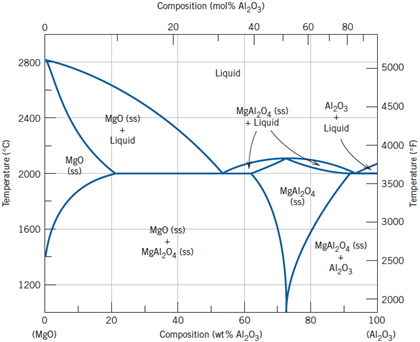
\includegraphics[width=250pt]{pics/p1_image.png}};
\node at (1.9,5) {\textbf{1}};
\node at (2.6,6) {\textbf{2}};
\node at (4,7) {\textbf{3}};
\node at (8.05,5) {\textbf{4}};
\node at (5.3,5) {\textbf{5}};
\node at (1.6,7.3) {\textbf{6}};
\draw [<->] (5.3,6) -- (6,5.1);
\node at (5.2,6) {\textbf{7}};
\node at (6.6,5.3) {\textbf{8}};
\node at (4,4.1) {\textbf{9}};
\node at (6.7,4.1) {\textbf{10}};
\node at (8,4.1) {\textbf{11}};
\draw [<->] (8.05,6) -- (8.4,5.0);
\node at (8.05,6.15) {\textbf{12}};
\end{tikzpicture}
\caption{MgO-$\text{Al}_2 \text{O}_3$ phase diagram.}
\end{figure}
\begin{center}
\begin{tabular}{c || c}
Position & Gibb's rule[1] \\ \hline
\textbf{1} & $F = 2 - 1 + 1 = 2$ \\ \hline
\textbf{2} &$F = 2 - 2 + 1 = 1$ \\ \hline
\textbf{3} &$F = 2 - 1 + 1 = 2$ \\ \hline
\textbf{4} &$F = 2 - 3 + 1 = 0$ \\ \hline
\textbf{5} &$F = 2 - 3 + 1 = 0$ \\ \hline
\textbf{6} &$F = 1 - 2 + 1 = 0$ \\ \hline
\textbf{7} &$F = 2 - 2 + 1 = 1$ \\ \hline
\textbf{8} &$F = 2 - 2 + 1 = 0$ \\ \hline
\textbf{9} &$F = 2 - 2 + 1 = 1$ \\ \hline
\textbf{10} &$F = 2 - 1 + 1 = 2$ \\ \hline
\textbf{11} &$F = 2 - 2 + 1 = 1$ \\ \hline
\textbf{12} &$F = 2 - 2 + 1 = 1$ \\ \hline
\end{tabular}
\end{center}

\begin{problem}{9.15}
Repeat Problem 9.14 for a 35:65 brass. \\
Reference: \textbf{9.14} Describe qualitatively the microstructural development during the slow cooling of a 30:70 brass (Cu with 30 wt\% Zn). See Figure 9.28 for the Cu-Zn phase diagram.
\end{problem}

\begin{figure}[H]
\centering
\begin{tikzpicture}

\node at (5,5) {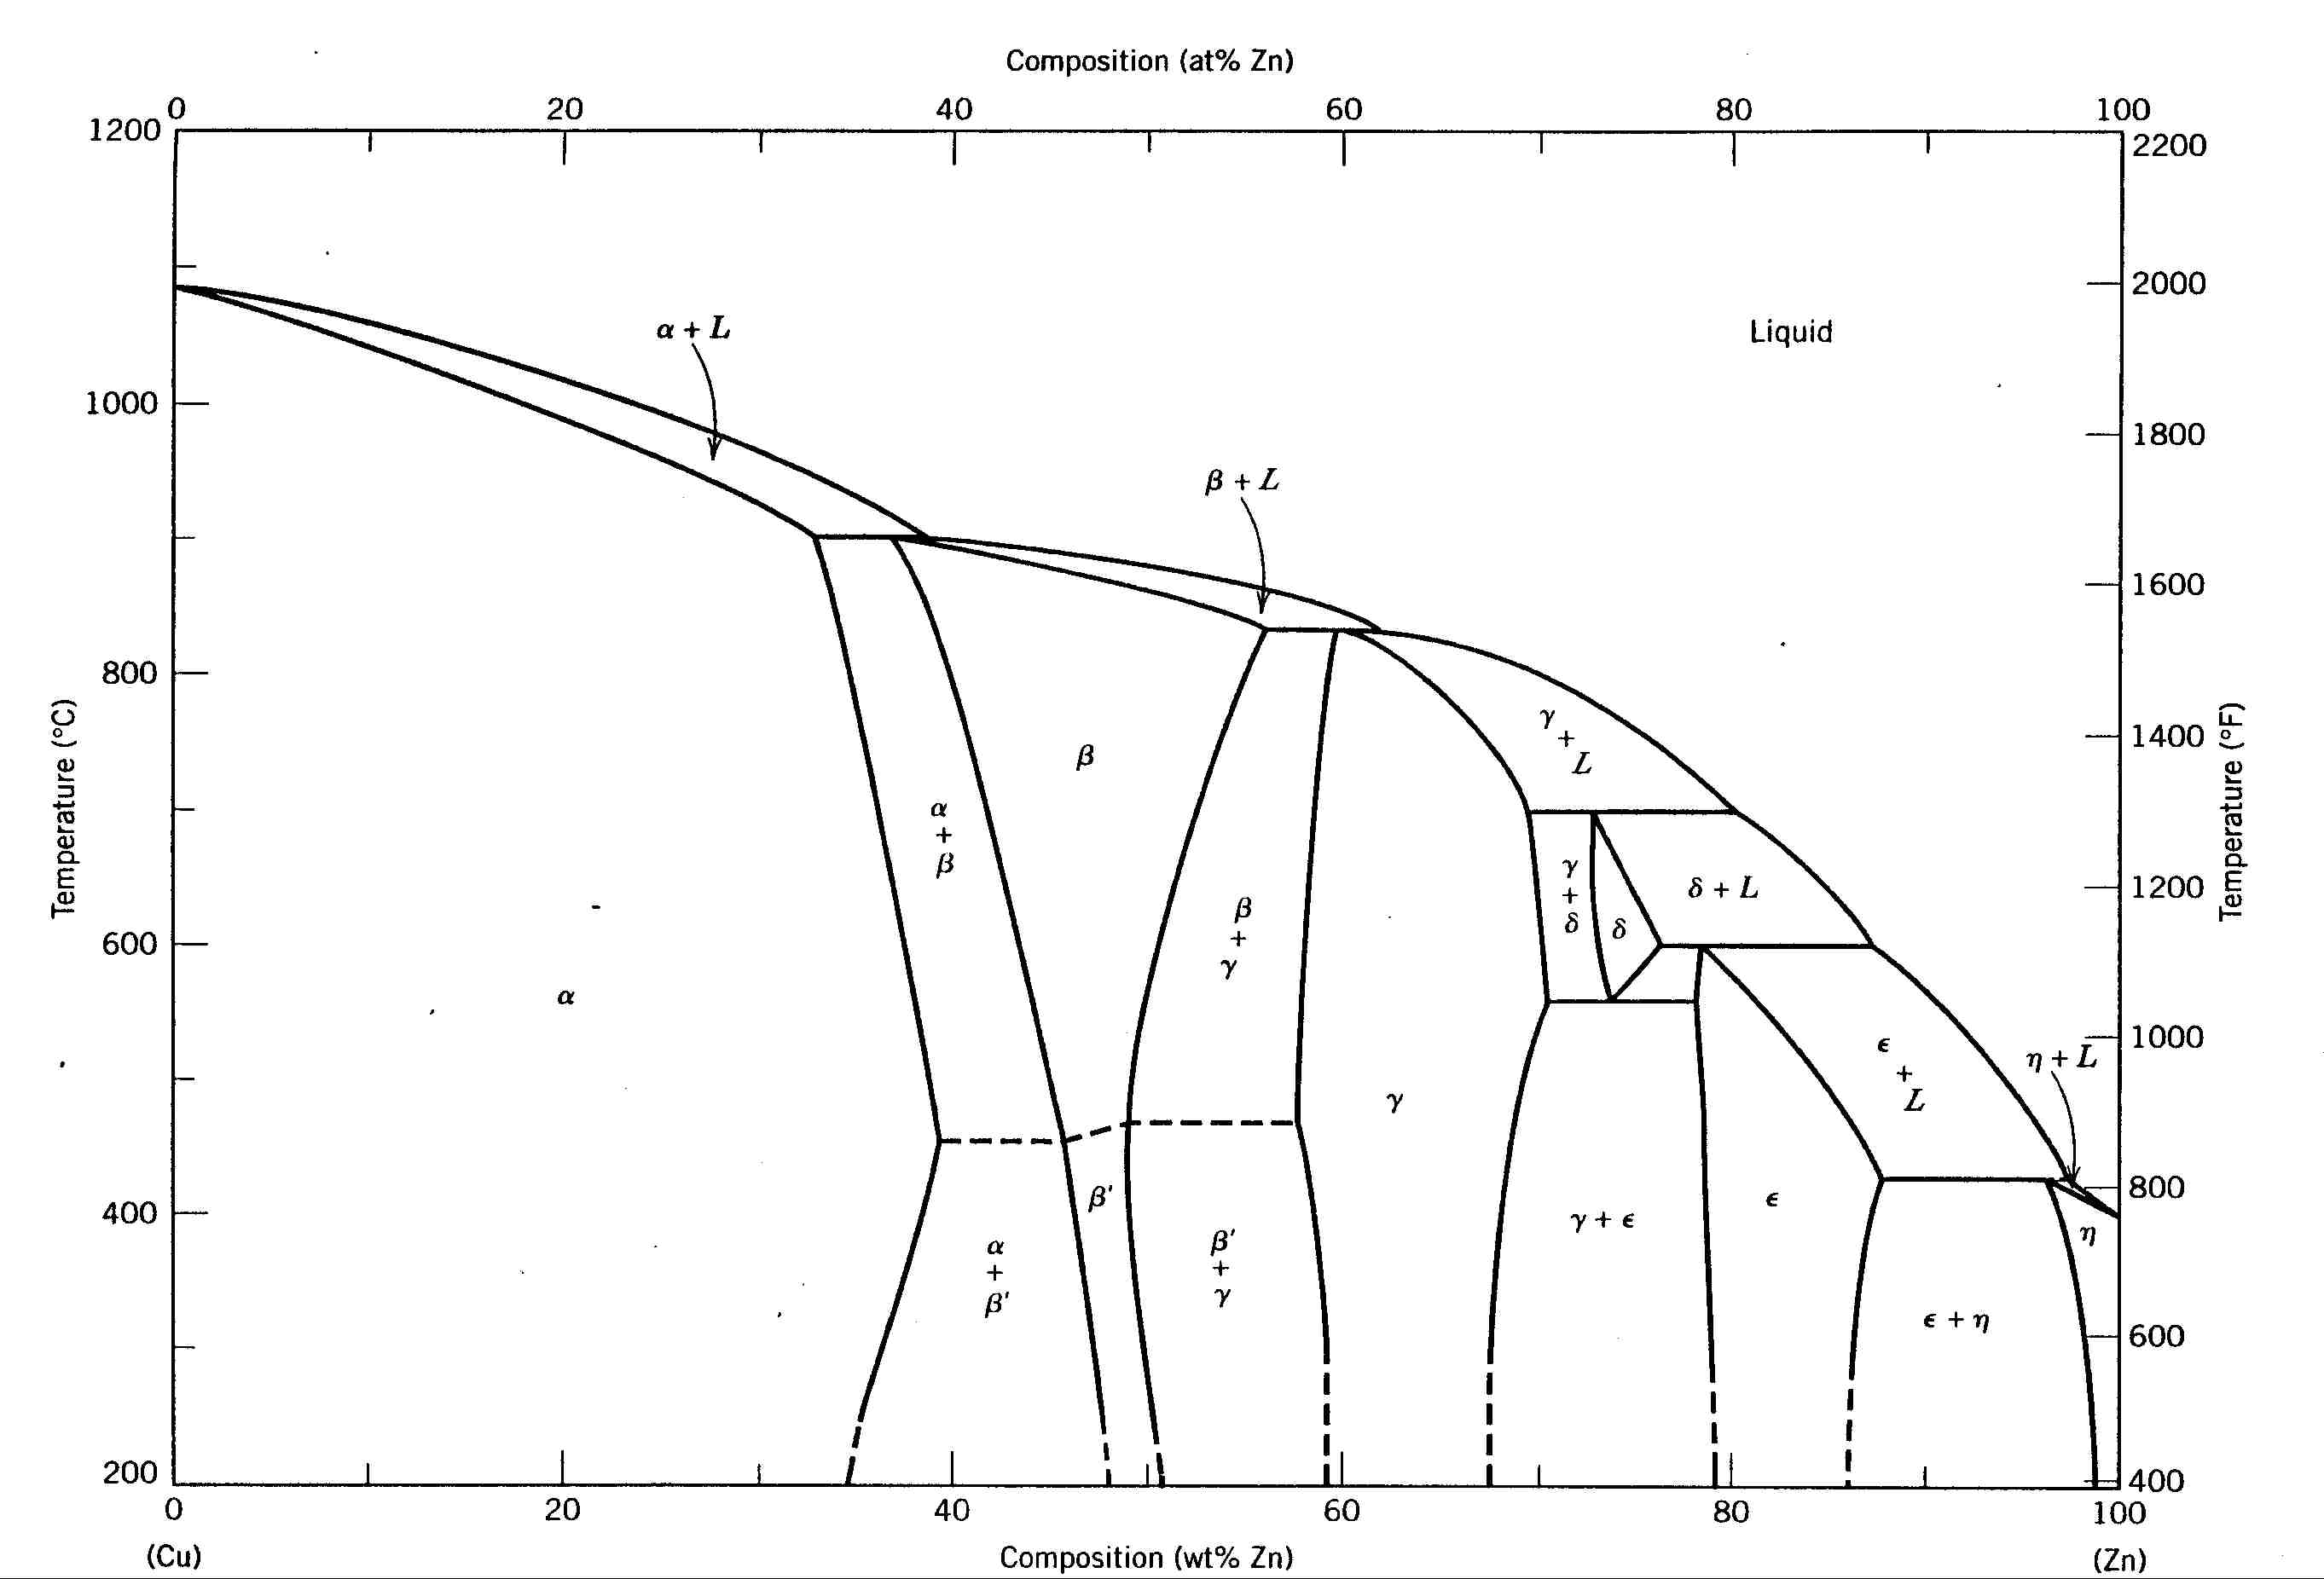
\includegraphics[width=400pt]{pics/p2_image.jpg}};
\draw[dashed,red] (3.2,8) -- (3.2,0);

\end{tikzpicture}
\caption{phase diagram for Cu-Zn [2]}
\end{figure}
Initially the micro structure is all liquid. As you cool down to $920\degree$C, you start to form crystallites of $\alpha$ inside the liquid. As you continue to cool down, right before you hit $903\degree$C there should be roughly $50\%$ $\alpha$ crystallites in the liquid as you are in the $\alpha + L$ phase. Below $903\degree$C you are now in the $\alpha + \beta$ region where the microstructure is eutectoid with fine alternating layers of $\alpha$ and $\beta$, and no more liquid is present anymore. As the temperature goes down in this region, the $\alpha$ lines become thicker while the $\beta$ lines become thinner. Eventually at a temperature of about $675\degree$C we enter the alpha region where our microstructure is now a polycrystalline solid of $\alpha$ and contains no more solid $\beta$. At a temperature of $200\degree$C we exit the $\alpha$ region and re-enter the $\alpha + \beta$ region where we now again have fine layered alternating lines of solid $\alpha$ and $\beta$. This is the region we stay at until the temperature is cooled to $0\degree$C.

\begin{problem}{9.25}
Suppose that you have a crucible containing 1 kg of an alloy of composition 90 wt\% Sn - 10 wt \% Pb at a temperature of $184\degree$C. How much Sn would you have to add to the crucible to completely solidify the alloy without changing the system temperature? (See Figure 9.16.)
\end{problem}
So initally we have 90\% tin in our solution. In order to solidify, and according to fig 9.16 in the book [1], we need 97.5\% tin. So this can be solved with a simple ratio.

\begin{align*}
\frac{0.9\text{kg} + x}{1\text{kg} + x} = 0.975 \\
(0.9 + x) = (1 + x)0.975 \\
0.9 - 0.975 = x0.975 - x \\
-0.075 = x(0.975 - 1) \\
-0.075 = -0.025x \\
x = \frac{0.075}{0.025} \\ 
x = 3\text{kg}
\end{align*}

\begin{problem}{9.35}
In a materials laboratory experiment, a student sketches a microstructure observed under an optical microscope. The sketch appears as \\
\begin{center}
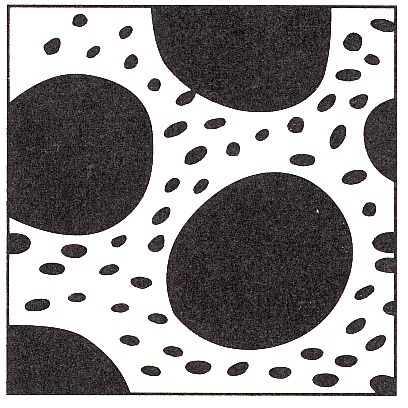
\includegraphics[width=250pt]{pics/p9_35_im1.jpg} \\
The phase diagram for this alloy is \\
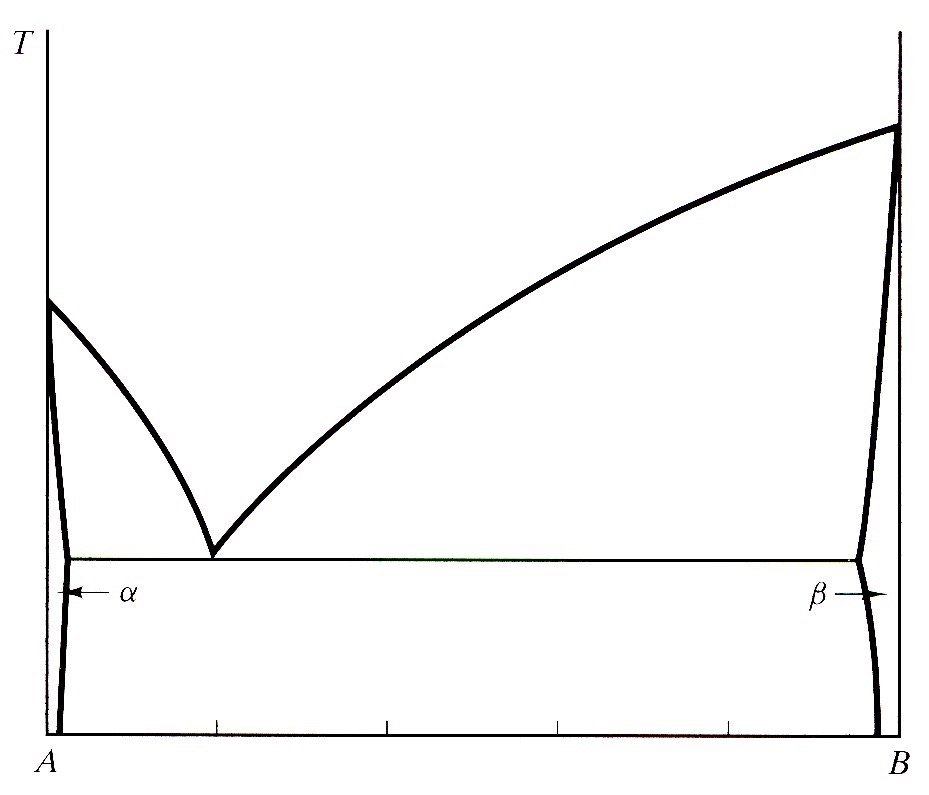
\includegraphics[width=250pt]{pics/p9_35_im2.jpg} \\
\end{center}
Determine \textbf{(a)} whether the black regions in the sketch represent alpha or beta phase and \textbf{(b)} the approximate alloy composition.
\end{problem}
\textbf{(a)} The small pieces of sloid in the picture indicates that the sketch is near the eutectic region as well as near the liquidus line. Since the eutectic point is near the alpha region, this leaves a large amount of area for the beta + liquid phase. This means that the sketch must be in the $\beta$ + L phase. \\
\textbf{(b)} The sketch shows the amount of $\beta$ and liquid phase. Guessing from looking at the sketch, the solid takes up about 50-60\% of the area while the liquid takes up the rest. So the sketch has about 60\% $\beta$ phase.

\begin{problem}{9.45}
Plot the weight percent of phases present as a function of temperature from 1,000 to 0$\degree$C for the 0.77 wt \% C eutectoid steel illustrated in Figure 9.38.
\end{problem}

\begin{figure}[H]
\centering
\begin{tikzpicture}
\node at (5,5) {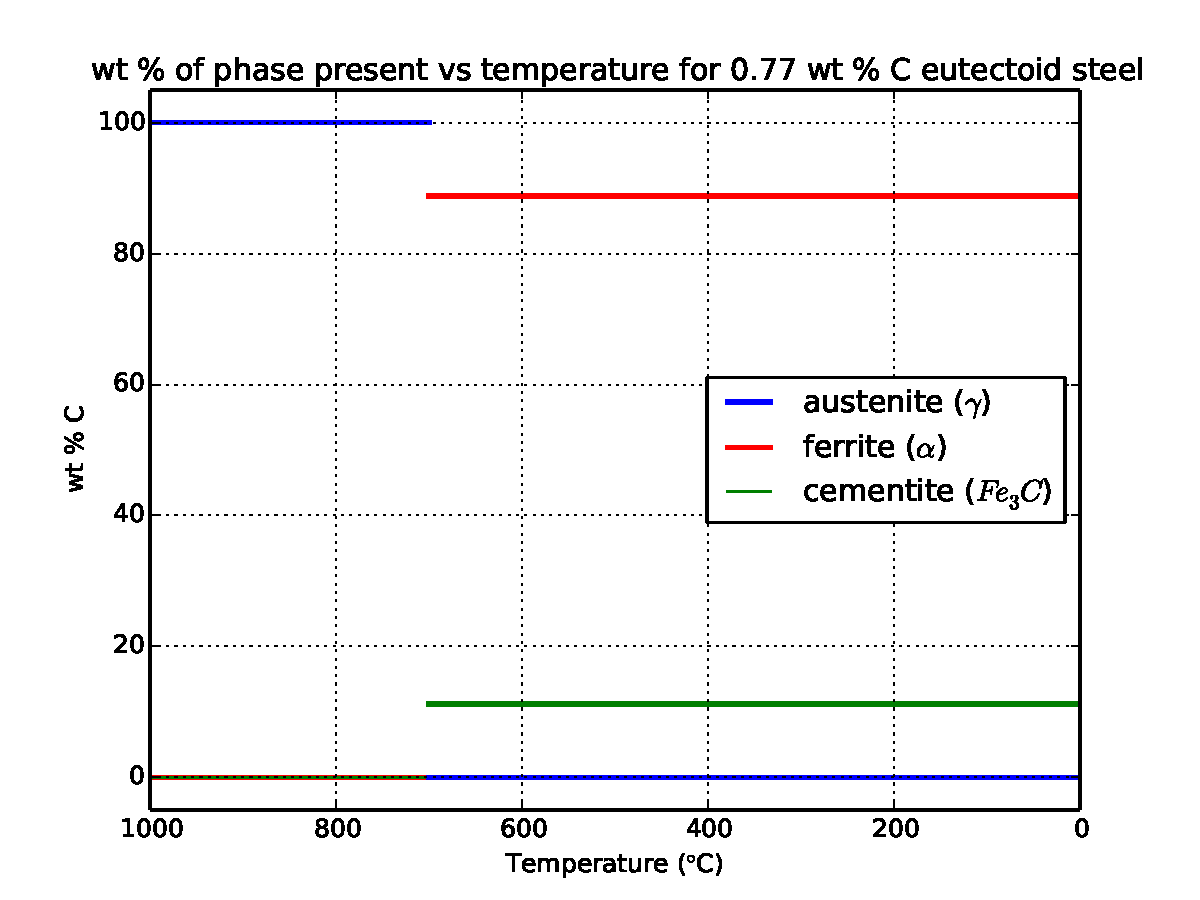
\includegraphics[width=350pt]{graphs/p9_45.pdf}};
\draw[dashed] (3.25,8.5) -- (3.25,1);
\node at (3.25,0.8) {$700$};
\node at (7,8) {88.8 \%};
\node at (7,2.7) {11.2 \%};
\end{tikzpicture}
\caption{The dashed $700\degree$C line represents the eutectic point in an Fe-F$\text{e}_3$C phase diagram. The lines after the eutectic point are in the $\alpha$ + $\text{Fe}_3$C region. Using the lever rule in that region, we can calculate the percentage of fermite and cementite in the phase: $m_{\alpha} = (x_{ss} - x)/(x_{ss} - x_l) = (6.7-0.77)/(6.7-0.02) = 0.888$. $m_{\text{Fe}_3 C} = 1 - m_{\alpha} = 0.112$.}
\end{figure}

\section{References}
\begin{enumerate}
\item James F. Shackelford, Introduction to Materials Science for Engineers, Seventh Edition, Pearson Higher 
Education, Inc., Upper Saddle River, New Jersey (2009).
\item "Zn." Aktüel Resim. AktuelResim.com, n.d. Web. 20 Oct. 2014.
\end{enumerate}




% --------------------------------------------------------------
%     You don't have to mess with anything below this line.
% --------------------------------------------------------------
 
\end{document}
